%preamble - package unclusion and set up
\documentclass[12pt,twoside,a4paper]{report}

% Select encoding of your inputs
\usepackage[utf8]{inputenc}

% Make latex understand and use the typographic
% rules of the language used in the document.
\usepackage[english]{babel}

% Use the vector font Latin Modern which is going
% to be the default font in latex in the future.
\usepackage{lmodern}

% Choose the font encoding
\usepackage[T1]{fontenc}

% Use color in tables
\usepackage[table]{xcolor}
\usepackage{array}
\usepackage{multirow}

% Load a colour package
\usepackage{xcolor}
\definecolor{aaublue}{RGB}{33,26,82}  %<--define aaublue
\definecolor{white}{RGB}{255,255,255} %<--define white

% The standard graphics inclusion package
\usepackage{graphicx}

\makeatletter
  \g@addto@macro\@floatboxreset\centering %<--centering all figures
\makeatother

\usepackage{adjustbox}

% Set up how figure and table captions are displayed
\usepackage{float}
\usepackage{caption}
\usepackage{subcaption}
\captionsetup
{
  justification = centering,    %<--centering caption with multiple lines
  font          = footnotesize, %<--set font size to footnotesize
  labelfont     = bf            %<--bold label (e.g., Figure 3.2) font
}
\captionsetup[subfigure]
{
  justification = centering, %<--centering subfigure caption text
  singlelinecheck=false,
  font = footnotesize        %<--font size for subfigures
} 

% Enable row combination in tables
\usepackage{multirow}

% Make space between table lines and text
\renewcommand{\arraystretch}{1.5}

% Enable commands like \st (strike out) and \hl (high light)
\usepackage{soul}

% Make the standard latex tables look so much better
\usepackage{array,booktabs}

% Enable the use of frames around, e.g., theorems
% The framed package is used in the example environment
\usepackage{framed}
\usepackage{colortbl}
\usepackage{longtable}
\usepackage{xcolor}
\usepackage{textcomp}

%-------MATHEMATICS---------------------------------
% Defines new environments such as equation,
% align and split 
\usepackage{amsmath}
\usepackage{relsize}
% Adds new math symbols
\usepackage{amssymb}
% Use theorems in your document
% The ntheorem package is also used for the example environment
% When using thmmarks, amsmath must be an option as well. Otherwise \eqref doesn't work anymore.
\usepackage[framed,amsmath,thmmarks]{ntheorem}
\usepackage{xifthen}%<--enables ifthenelse which is used in macros

\usepackage{siunitx} 
\sisetup{decimalsymbol=period}%<--\num{} will swich commas with periods
\sisetup{detect-weight}
%---------------------------------------------------

%-------PAGE LAYOUT---------------------------------
% Change margins, papersize, etc of the document
\usepackage[
  left=25mm,% left margin on an odd page %tidligere 25mm for baade right og left
  right=25mm,% right margin on an odd page
  top=35mm,
  ]{geometry}
  
% Modify how \chapter, \section, etc. look
% The titlesec package is very configureable
\usepackage{titlesec}
\makeatletter
\def\ttl@mkchap@i#1#2#3#4#5#6#7{%
    \ttl@assign\@tempskipa#3\relax\beforetitleunit
    \vspace{\@tempskipa}%<<<<<< REMOVE THE * AFTER \vspace
    \global\@afterindenttrue
    \ifcase#5 \global\@afterindentfalse\fi
    \ttl@assign\@tempskipb#4\relax\aftertitleunit
    \ttl@topmode{\@tempskipb}{%
        \ttl@select{#6}{#1}{#2}{#7}}%
    \ttl@finmarks  % Outside the box!
    \@ifundefined{ttlp@#6}{}{\ttlp@write{#6}}}
\makeatother

\titlespacing{\chapter}{0pt}{0pt}{10pt}
\titlespacing{\section}{0pt}{0pt}{-5pt}
\titlespacing{\subsection}{0pt}{8pt}{-5pt}
\titlespacing{\subsubsection}{0pt}{6pt}{-10pt}

\titleformat*{\section}{\normalfont\Large\bfseries\color{aaublue}}
\titleformat*{\subsection}{\normalfont\large\bfseries\color{aaublue}}
\titleformat*{\subsubsection}{\normalfont\normalsize\bfseries\color{aaublue}}

\usepackage{titlesec, blindtext, color}
%\color{gray75}{gray}{0.75}
\newcommand{\hsp}{\hspace{20pt}}
\titleformat{\chapter}[hang]{\Huge\bfseries}{\thechapter\hsp\textcolor{aaublue}{|}\hsp}{0pt}{\Huge\bfseries}

% Change the headers and footers
\usepackage{fancyhdr}
\setlength{\headheight}{15pt}
\pagestyle{fancy}
\fancyhf{} %delete everything
\renewcommand{\headrulewidth}{0pt} %remove the horizontal line in the header
\fancyhead[RO,LE]{\color{aaublue}\small\nouppercase\leftmark} %even page - chapter title
\fancyhead[LO]{}
\fancyhead[RE]{} 
\fancyhead[CE]{}
\fancyhead[CO]{}
\fancyfoot[RE,LO]{\thepage}
\fancyfoot[LE,RO]{} %page number on all pages
\fancyfoot[CE,CO]{}

% change first page of all chapters header and footer to fancy style
\makeatletter
\let\ps@plain\ps@fancy
\makeatother

% Do not stretch the content of a page. Instead,
% insert white space at the bottom of the page
\raggedbottom

% Enable arithmetics with length. Useful when typesetting the layout.
\usepackage{calc}
%---------------------------------------------------

%-------BIBLIOGRAPHY--------------------------------
%setting references (using numbers) and supporting i.a. Chicargo-style:
\usepackage{etex}
\usepackage{etoolbox}
\usepackage{keyval}
\usepackage{ifthen}
\usepackage{url}
\usepackage{csquotes}
\usepackage[backend=biber, url=true, doi=true, style=numeric, sorting=none]{biblatex}
\addbibresource{setup/bibliography.bib}
%---------------------------------------------------

%-------MISC----------------------------------------
%%% Enables the use FiXme refferences. Syntax: \fxnote{...} %%%
\usepackage[footnote, draft, english, silent, nomargin]{fixme}
%With "final" instead of "draft" an error will ocure for every FiXme under compilation.

%%% allows use of lorem ipsum (generate i.e. pagagraph 1 to 5 with \lipsum[1-5]) %%%
\usepackage{lipsum}

%%% Enables figures with text wrapped tightly around it %%%
\usepackage{wrapfig}

%%% Section debth included in table of contents (1 = down to sections) %%%
\setcounter{tocdepth}{1}

%%% Section debth for numbers (1 = down to sections) %%%
\setcounter{secnumdepth}{1}

\usepackage{tocloft}
\setlength{\cftbeforetoctitleskip}{0 cm}
\renewcommand{\cftpartpresnum}{Part~}
\let\cftoldpartfont\cftpartfont
\renewcommand{\cftpartfont}{\cftoldpartfont\cftpartpresnum}
%---------------------------------------------------

%-------HYPERLINKS----------------------------------
% Enable hyperlinks and insert info into the pdf
% file. Hypperref should be loaded as one of the 
% last packages
\usepackage{nameref}
\usepackage{hyperref}
\hypersetup{%
	%pdfpagelabels=true,%
	plainpages=false,%
	pdfauthor={Author(s)},%
	pdftitle={Title},%
	pdfsubject={Subject},%
	bookmarksnumbered=true,%
	colorlinks,%
	citecolor=aaublue,%
	filecolor=aaublue,%
	linkcolor=aaublue,% you should probably change this to black before printing
	urlcolor=aaublue,%
	pdfstartview=FitH%
}
%---------------------------------------------------

% remove all indentations
\setlength\parindent{0pt}
\parskip 5mm
\usepackage{verbatim}

\definecolor{Gra}{RGB}{230,230,230}

%creates a nice-looking C#-text
\newcommand{\CC}{C\nolinebreak\hspace{-.05em}\raisebox{.3ex}{\scriptsize\text \#} }

%enables multi column lists
\usepackage{multicol}



%enables code-examples
\usepackage{listings}

\definecolor{coolblue}{RGB}{32,95,128}
\definecolor{mygreen}{rgb}{0,0.6,0}
\definecolor{mygray}{rgb}{0.5,0.5,0.5}
\definecolor{mymauve}{rgb}{0.58,0,0.82}
\usepackage{textcomp}
\definecolor{listinggray}{gray}{0.9}
\definecolor{lbcolor}{rgb}{0.9,0.9,0.9}

\lstdefinestyle{pythonstyle}{
    backgroundcolor=\color{lbcolor},
    tabsize=4,
    rulecolor=,
    language=python,
    basicstyle=\scriptsize,
    upquote=true,
    aboveskip={1.5\baselineskip},
    columns=fixed,
    showstringspaces=false,
    extendedchars=true,
    breaklines=true,
    prebreak = \raisebox{0ex}[0ex][0ex]{\ensuremath{\hookleftarrow}},
    frame=single,
    showtabs=false,
    numbers=left,
    captionpos=b,
    numbersep=5pt,
    numberstyle=\tiny\color{mygray},
    showspaces=false,
    showstringspaces=false,
    identifierstyle=\ttfamily,
    keywordstyle=\color[rgb]{0,0,1},
    commentstyle=\color[rgb]{0.133,0.545,0.133},
    stringstyle=\color[rgb]{0.627,0.126,0.941},
}
\lstdefinestyle{custommatlab}{
    backgroundcolor=\color{lbcolor},
    tabsize=4,
    rulecolor=,
    language=Matlab,
    basicstyle=\scriptsize,
    upquote=true,
    aboveskip={1.5\baselineskip},
    columns=fixed,
    showstringspaces=false,
    extendedchars=true,
    breaklines=true,
    prebreak = \raisebox{0ex}[0ex][0ex]{\ensuremath{\hookleftarrow}},
    frame=single,
    showtabs=false,
    numbers=left,
    captionpos=b,
    numbersep=5pt,
    numberstyle=\tiny\color{mygray},
    showspaces=false,
    showstringspaces=false,
    identifierstyle=\ttfamily,
    keywordstyle=\color[rgb]{0,0,1},
    commentstyle=\color[rgb]{0.133,0.545,0.133},
    stringstyle=\color[rgb]{0.627,0.126,0.941},   
}
\lstdefinestyle{custommatlabinline}{
    style=custommatlab,
    basicstyle=\small,
}
\lstdefinestyle{pythoninline}{
    style=pythonstyle,
    basicstyle=\small,
}

%% Python for inline
\newcommand\pythonline[1]{ \lstinline[style=pythoninline]{#1} }

\usepackage{enumitem}
%\usepackage[citestyle=authoryear,natbib=true]{biblatex}

% Figures - TIKZ
\usepackage{tikz}
\usepackage[americanresistors,americaninductors,americancurrents, americanvoltages]{circuitikz}

% Wall of text logo
\newcommand{\walloftextalert}[0]{\includegraphics[width=\textwidth]{walloftext.png}}

\usepackage{pdfpages}
\usepackage{lastpage}
\usepackage{epstopdf}

\setlength{\headheight}{21pt}

\hfuzz=\maxdimen
\tolerance = 10000
\hbadness  = 10000

\usepackage{siunitx}
\graphicspath{{./figures/}}

%macros - please read this file
%Macro for 'where'-enviroment was improved by Andrea and Niels :-)

%-----------UNITS-------------------------------------------
\newcommand{\unit}[1]{&& \left[\si{#1}\right]}
%
%\newcommand{\unit}[1]{[\si{#1}]}            %<<| Use these if you want equations to be
%\newcommand{\eq}[2]{&&\si{#1} &= \si{#2}&&} %<<| centered.. .. will appear scrambled
%                                            %  | from one equation to the next though..
%                                            %  | and does not work with long equations.. :/
%
%-----------------------------------------------------------

%-----------WHERE ENVIRONMENT-------------------------------
\newenvironment{where}{\leavevmode{\parindent=1em\indent} Where:\\}{}
\newcommand{\va}[3]
{
  \begin{tabular}{p{20pt} p{40pt} p{290pt} l}
    & { $#1$ } & { #2 } & \ifthenelse{\isempty{ #3 }}  {}  {[{\si{#3}}]} \\
  \end{tabular}\\
}
%-----------------------------------------------------------

%-----------TikZ SETTINGS-----------------------------------
\tikzset{
  block/.style    = {draw, thick, rectangle,
                     minimum height = 2.1em,
                     minimum width = 1.7em},
  sum/.style      = {draw, circle, inner sep=3pt} %<--Adder
}
%----------------------------------------------------------- %TIP: If you are using TeXstudio you can open
                         %     the file by Ctrl+LeftClick on setup/macros.tex

\begin{document}
\section*{Model Predictive Control Exercise - Group 17gr832}
Alejandro Alonso García\\
Anders Egelund Kjeldal\\
Himal Kooverjee  \\
Niels Skov Vestergaard\\
Noelia Villarmarzo Arruñada
%
\subsection*{Description of the Problem}
The objective is to optimize the profit that can be obtained by running the plant showed in \autoref{fig:powerPlant}.

\begin{figure}[H]
    \centering
    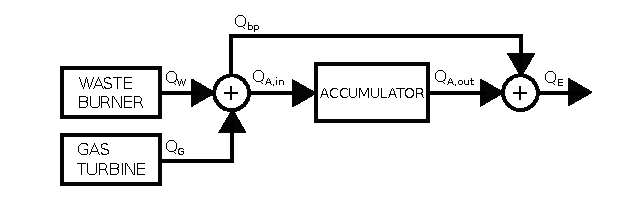
\includegraphics[width=0.6\textwidth]{figures/powerPlant}
    \caption{Diagram of the plant, where $Q_\mathrm{G}$ is the power produced by the gas turbine, $Q_\mathrm{W}$ is the power produced by the waste burner, $Q_\mathrm{A,in}$ is the power fed into the accumulator, $Q_\mathrm{bp}$ is the power bypassing the accumulator, $Q_\mathrm{A,out}$ is the power leaving the accumulator, and $Q_\mathrm{E}$ is the power leaving the plant. The units of power are given in megawatt [MW]}
    \label{fig:powerPlant}
\end{figure}

The power flows in the plant have some constraints shown below:
%
\begin{flalign}
    Q_\mathrm{W} + Q_\mathrm{G} = Q_\mathrm{bp} + Q_\mathrm{A,in}, \ \ & \ \ Q_\mathrm{E} = Q_\mathrm{bp} + Q_\mathrm{A,out} \label{eq:equality} \\
    0 \leq Q_\mathrm{W} \leq 40, \ \  \ \  0 \leq Q_\mathrm{G} \leq 20 \ \ & \ \ 0, \leq Q_\mathrm{A,in} \leq 50, \ \  \ \ 0 \leq Q_\mathrm{A,out} \leq 25 \label{eq:inequality}
\end{flalign}

And the accumulator have some dynamics and some constraints as well
%
\begin{flalign}
    &E_\mathrm{A}[k+1] = E_\mathrm{A}[k] + (Q_\mathrm{A,in}[k] - Q_\mathrm{A,out}[k]) T_\mathrm{s} \label{eq:dynamics}\\
    &0 \leq E_\mathrm{A} \leq 200 \label{eq:inequality_E}
\end{flalign}

The profit can be optimized by scheduling the power production using the knowledge of the plant and  the future prices of gas, waste burning and electricity ($P_\mathrm{G}$, $P_\mathrm{W}$ and $P_\mathrm{E}$). The profit is given by
%
\begin{flalign}
    \sum_{i=k}^{k+L-1} (P_\mathrm{E}[i] Q_\mathrm{E}[i] - (P_\mathrm{G}[i] Q_\mathrm{G}[i] + P_\mathrm{W}[i] Q_\mathrm{W}[i])) T_\mathrm{s} \label{eq:cost}
\end{flalign}

\subsection*{Problem Formulation in CVX Form}
Once the problem has been described, the constraints, the dynamic equation and the cost function need to be rewritten in a suitable way to be able to optimize the problem using CVX.

The dynamic equation, \autoref{eq:dynamics}, of the accumulator can be rewritten by substituting backwards each $E_\mathrm{A}[k]$ until it depends only on the inputs and the initial state.
%
\begin{flalign}
    E_\mathrm{A}[k+1] = E_\mathrm{A}[k] + &(Q_\mathrm{A,in}[k] - Q_\mathrm{A,out}[k]) T_\mathrm{s} \\
    &... \nonumber \\
    E_\mathrm{A}[k+l] = E_\mathrm{A}[k] + &\sum_{i=k}^{k+l-1}(Q_\mathrm{A,in}[i] - Q_\mathrm{A,out}[i]) T_\mathrm{s} \\
    &... \nonumber \\
    E_\mathrm{A}[k+L] = E_\mathrm{A}[k] + &\sum_{i=k}^{k+L-1}(Q_\mathrm{A,in}[i] - Q_\mathrm{A,out}[i]) T_\mathrm{s}
\end{flalign}

This expression can also be rewritten in matrix form as follows
\begin{flalign}
    \begin{bmatrix}
        E_\mathrm{A}[k+1] \\
        E_\mathrm{A}[k+2] \\
        ...\\
        E_\mathrm{A}[k+L] \\
    \end{bmatrix}
    =  
    \begin{bmatrix}
        E_\mathrm{A}[k] \\
        E_\mathrm{A}[k] \\
        ...\\
        E_\mathrm{A}[k] \\
    \end{bmatrix}  
    +
    \begin{bmatrix}
        Q_\mathrm{A,in}[k] - Q_\mathrm{A,out}[k] \\
        Q_\mathrm{A,in}[k+1] - Q_\mathrm{A,out}[k+1] \\
        ... \\
        Q_\mathrm{A,in}[k+L-1] - Q_\mathrm{A,out}[k+L-1]
    \end{bmatrix}^\mathrm{T}
    \begin{bmatrix}
        1 & 1 & 1 & ... & 1 \\
        0 & 1 & 1 & ... & 1\\
        0 & 0 & 1 & ... & 1\\
        ... & ... & ... & ... & ... \\
        0 & 0 & 0 & ... & 1
    \end{bmatrix} \label{eq:matrix_dynamics}
\end{flalign}

Since there exists a constraint on the amount of charge that can be stored in the accumulator at each time, \autoref{eq:matrix_dynamics} can be used to write that constraint in an appropriate form.
\begin{flalign}
    0 \leq  
    \begin{bmatrix}
        E_\mathrm{A}[k] \\
        E_\mathrm{A}[k] \\
        ...\\
        E_\mathrm{A}[k] \\
    \end{bmatrix}  
    +
    \begin{bmatrix}
        Q_\mathrm{A,in}[k] - Q_\mathrm{A,out}[k] \\
        Q_\mathrm{A,in}[k+1] - Q_\mathrm{A,out}[k+1] \\
        ... \\
        Q_\mathrm{A,in}[k+L-1] - Q_\mathrm{A,out}[k+L-1]
    \end{bmatrix}^\mathrm{T}
    \begin{bmatrix}
        1 & 1 & 1 & ... & 1 \\
        0 & 1 & 1 & ... & 1\\
        0 & 0 & 1 & ... & 1\\
        ... & ... & ... & ... & ... \\
        0 & 0 & 0 & ... & 1
    \end{bmatrix}
    \leq 200 \label{eq:matrix_constraint}
\end{flalign}

The equality constraints in \autoref{eq:equality} can be used to rewrite the cost function, \autoref{eq:cost}, as a function of $Q_\mathrm{G}$, $Q_\mathrm{W}$, $Q_\mathrm{A,in}$ and $Q_\mathrm{A,out}$. This results in \autoref{eq:final_cost}
%
\begin{flalign}
    & \sum_{i=k}^{k+L-1} (P_\mathrm{E}[i] Q_\mathrm{E}[i] - (P_\mathrm{G}[i] Q_\mathrm{G}[i] + P_\mathrm{W}[i] Q_\mathrm{W}[i])) T_\mathrm{s} \\
    & \sum_{i=k}^{k+L-1} (P_\mathrm{E}[i] (Q_\mathrm{bp}[i] + Q_\mathrm{A,out}[i]) - (P_\mathrm{G}[i] Q_\mathrm{G}[i] + P_\mathrm{W}[i] Q_\mathrm{W}[i])) T_\mathrm{s} \\
    & \sum_{i=k}^{k+L-1} (P_\mathrm{E}[i] (Q_\mathrm{W}[i] + Q_\mathrm{G}[i] - Q_\mathrm{A,in}[i] + Q_\mathrm{A,out}) - (P_\mathrm{G}[i] Q_\mathrm{G}[i] + P_\mathrm{W}[i] Q_\mathrm{W}[i])) T_\mathrm{s} \\
    & \sum_{i=k}^{k+L-1} ((P_\mathrm{E}[i] - P_\mathrm{W}[i])Q_\mathrm{G}[i] + (P_\mathrm{E}[i] - P_\mathrm{G}[i])Q_\mathrm{G}[i] + P_\mathrm{E}[i] Q_\mathrm{A,out}[i] - P_\mathrm{E}[i] Q_\mathrm{A,in}[i]) T_\mathrm{s} \label{eq:final_cost}
\end{flalign}

This expression can also be written in matrix form to be suitable to use with CVX.
\footnotesize{
\begin{flalign}
    \begin{bmatrix}
        P_\mathrm{E}[k] - P_\mathrm{W}[k] \\
        P_\mathrm{E}[k+1] - P_\mathrm{W}[k+1] \\
        ...\\
        P_\mathrm{E}[k+L-1] -P_\mathrm{W}[k+L-1] \\
    \end{bmatrix}^\mathrm{T}  
    \begin{bmatrix}
        Q_\mathrm{W}[k] \\
        Q_\mathrm{W}[k+1] \\
        ...\\
        Q_\mathrm{W}[k+L-1] \\
    \end{bmatrix}  
    +
    \begin{bmatrix}
        P_\mathrm{E}[k] - P_\mathrm{G}[k] \\
        P_\mathrm{E}[k+1] - P_\mathrm{G}[k+1] \\
        ...\\
        P_\mathrm{E}[k+L-1] -P_\mathrm{G}[k+L-1] \\
    \end{bmatrix}^\mathrm{T}  
    \begin{bmatrix}
        Q_\mathrm{G}[k] \\
        Q_\mathrm{G}[k+1] \\
        ...\\
        Q_\mathrm{G}[k+L-1] \\
    \end{bmatrix}
    + \nonumber\\
    +
    \begin{bmatrix}
        P_\mathrm{E}[k] \\
        P_\mathrm{E}[k+1]\\
        ...\\
        P_\mathrm{E}[k+L-1]\\
     \end{bmatrix}^\mathrm{T}  
     \begin{bmatrix}
         Q_\mathrm{A_out}[k] \\
         Q_\mathrm{A_out}[k+1] \\
         ...\\
         Q_\mathrm{A_out}[k+L-1] \\
     \end{bmatrix}  
     -
     \begin{bmatrix}
         P_\mathrm{E}[k]\\
         P_\mathrm{E}[k+1]\\
         ...\\
         P_\mathrm{E}[k+L-1]\\
     \end{bmatrix}^\mathrm{T}  
     \begin{bmatrix}
         Q_\mathrm{A_in}[k] \\
         Q_\mathrm{A_in}[k+1] \\
         ...\\
         Q_\mathrm{A_in}[k+L-1] \\
     \end{bmatrix}\label{eq:matrix_cost}
\end{flalign}
}
\normalsize
\subsection*{Implementation}
The implementation of the optimization problem is shown in \autoref{cvxImplementation}. It includes the inequality constraints in \autoref{eq:inequality} and \ref{eq:matrix_constraint} as well as the cost defined in \autoref{eq:matrix_cost}.
%
\begin{lstlisting}[ language = Matlab,
					caption  = {MATLAB code for the implementation of the problem with CVX},
					label    = cvxImplementation ]
cvx_begin quiet % The beginning of the optimization problem

    % Define the variables
    variable Q_W(L,1);
    variable Q_G(L,1);
    variable Q_A_in(L,1);
    variable Q_A_out(L,1);
    
    % Specify the optimization of cost
    minimize(-(P_E(k:k+L-1)'*Q_A_out+(P_E(k:k+L-1)'-P_G(k:k+L-1)')*Q_G+...
    (P_E(k:k+L-1)'-P_W(k:k+L-1)')*Q_W-P_E(k:k+L-1)'*Q_A_in)*Ts);
    
    % Constraints
    subject to 
    Q_W>=Q_W_min;
    Q_W<=Q_W_max;
    Q_G>=Q_G_min;
    Q_G<=Q_G_max;
    Q_A_in>=Q_A_in_min;
    Q_A_in<=Q_A_in_max;
    Q_A_out>=Q_A_out_min;
    Q_A_out<=Q_A_out_max;
    (Q_A_in-Q_A_out)'*triu(ones(L,L))>=E_A_min-E_A_sys(k);
    (Q_A_in-Q_A_out)'*triu(ones(L,L))<=E_A_max-E_A_sys(k);
    
cvx_end     % The end of the optimization problem
\end{lstlisting}

In each iteration of the loop it tries to minimize the cost along the horizon $L$ knowing the corresponding prices and the inequality constraints, by finding the optimal $Q_\mathrm{W}$, $Q_\mathrm{W}$, $Q_\mathrm{A,in}$ and $Q_\mathrm{A,out}$.

\subsection*{Results}
The results obtained are presented in \autoref{fig:E_A}, \ref{fig:Q_E}, \ref{fig:Q_W} and \ref{fig:Q_G}.

In \autoref{fig:E_A} the state of charge of the accumulator can be seen. It shall be noticed that the accumulator charges when the price of electricity is low and discharges when it is high. For this to be seen it is neccesary to look also at \autoref{fig:Q_E}, where the power production and price is depicted. Good examples appear at 90 hours and between 170 and 180 hours. The accumulator also charges when the power production of gas is cheaper, this is shown in \autoref{fig:Q_G}. The clearest example of this occurs between 110 and 120 hours.

From the power production seen in \autoref{fig:Q_E}, it can be said that the power produced is low when electricity is cheap and high otherwise. This is clear in the graph as when the price peaks up, so does the production and vice versa
\begin{figure}[H]
    \captionbox 
    {
    	State of charge in the accumulator.
        \label{fig:E_A}                                  
    }                                                                 
    {                                                                 
        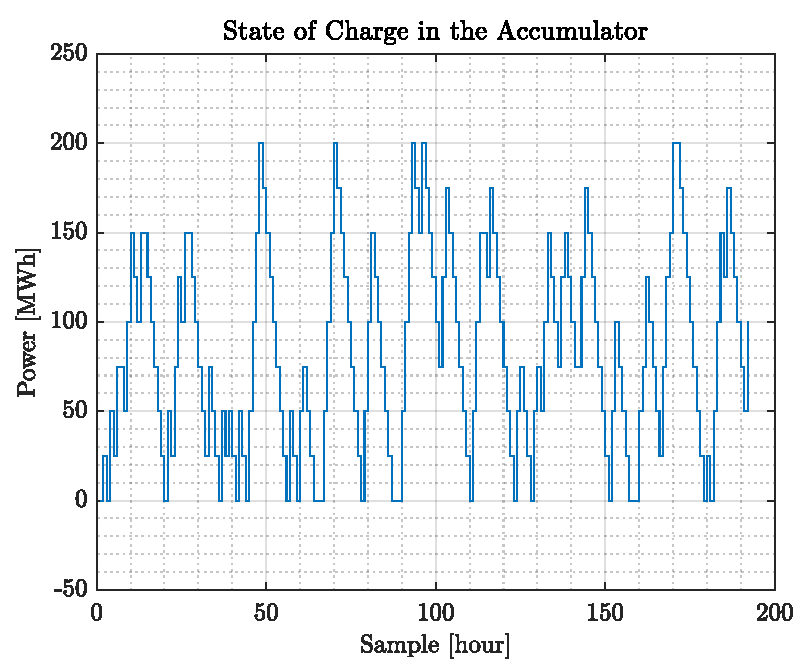
\includegraphics[height=.37\textwidth]{figures/E_A}
    }                                                                    
    \hspace{5pt}                                                          
    \captionbox  
    {        
        Comparison of the power production and the price of electricity.    
        \label{fig:Q_E}                                    
    }                                                                     
    {   
        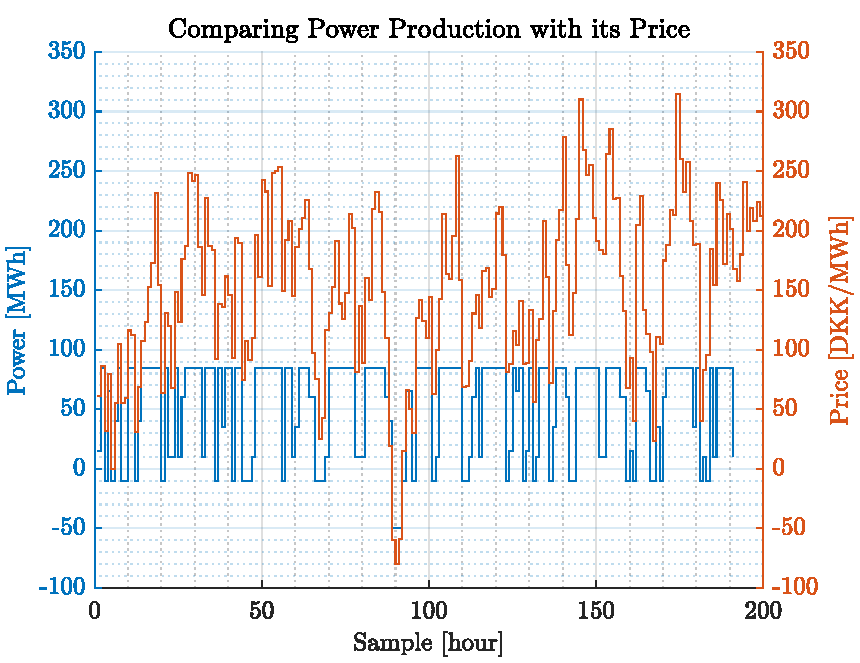
\includegraphics[height=.37\textwidth]{Q_E}            
    }                                                                             
\end{figure}
The information presented in \autoref{fig:Q_W} and \ref{fig:Q_G} shows how the electric power is produced. It can be observed how waste is used in almost all the simulation as its price is negative. The only exception occurs when the price of electricity is also negative. This leads to a stop in the electricity production and from gas and waste and a charging period of the accumulator using electric power from outside the plant. The use of gas is more interesting as it is used as long as its price is lower than that of electricity, else the production of electric power with gas is zero. Examples of this take place between 65 and 70 hours, between 90 and 95 hours and at 160 hours.
\begin{figure}[H]
    \captionbox
    {       
        Comparison of the power produced using waste and the price of waste burning.          
        \label{fig:Q_W}                                  
    }                                                                 
    {                                                                  
        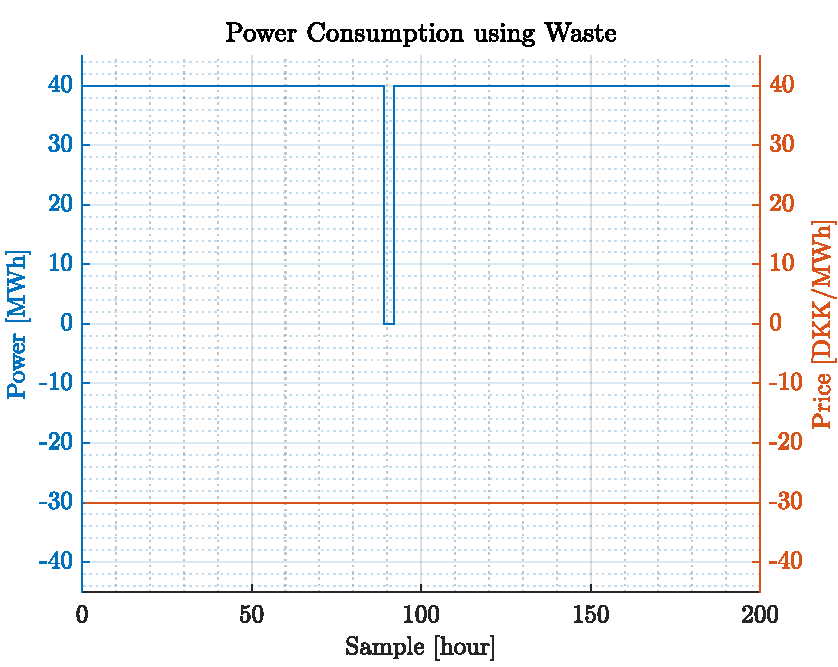
\includegraphics[height=.37\textwidth]{figures/Q_W} 
    }                                                                    
    \hspace{5pt}                                                          
    \captionbox  
    {          
        Comparison of the power produced using gas and the difference between the price of electricity and the price of gas.
        \label{fig:Q_G}                                     
    }                                                                     
    {                                                                     
        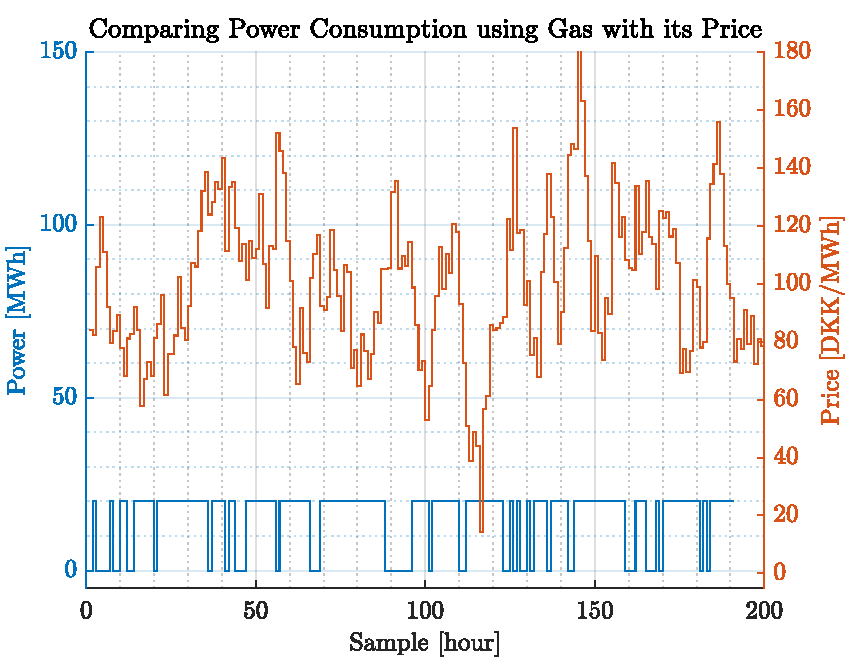
\includegraphics[height=.37\textwidth]{Q_G}            
    }      
\end{figure}
All the information presented suggests that the plant operates taking into account the different prices and adjusting the power production in order to maximize the profit obtained when running.
\end{document}
